\documentclass[AER]{AEA}

% --- 必须的宏包 ---
\usepackage{tikz}
\usetikzlibrary{shapes, arrows, positioning, fit, calc, backgrounds}
\usepackage{amsmath, amssymb}
\usepackage{booktabs}
\usepackage{lipsum}
\usepackage{placeins}
\usepackage{natbib} 

% --- 终极防伪：链接与字体设置 ---
\usepackage{url}
\usepackage{xcolor} 
\newcommand{\noopsort}[1]{} 
\DeclareRobustCommand{\AERlink}[1]{}
\usepackage[hidelinks]{hyperref}

\issueName{THE AMERICAN ECONOMIC RUBBISH}

% 草稿行距设置
\draftSpacing{1.5}

\begin{document}

% --- 封面信息 ---
% 1. 标题硬编码十字架
\title{Where is the Money? A Test of Intertemporal Monetary Neutrality in the ``Grandma-Managed'' Red Envelope Economy$^\dagger$}
\shortTitle{Where is the Money?}

% 2. 作者硬编码星号，彻底抛弃 \thanks，杜绝缩进错误
\author{Gemini and Sky Horse$^*$}

\date{\today}
\pubMonth{February}
\pubYear{2026}
\pubVolume{1}
\pubIssue{1}

\begin{abstract}
During the Chinese New Year, the nominal assets of juvenile agents experience a temporary stochastic shock known as ``Red Envelopes'' (Hongbao). However, empirical observation suggests that child consumption remains flat despite this wealth injection. We model the ``Mommy Deposit Facility'' (MDF) as a perfect liquidity sink. Using a dynamic stochastic general equilibrium (DSGE) model with imperfect parental credibility, we find that the marginal propensity to consume (MPC) out of Red Envelopes is statistically indistinguishable from zero. Our Impulse Response Function (IRF) analysis confirms that 100\% of the liquidity is absorbed by the ``I am saving it for your tuition'' mechanism, effectively creating a black hole in the household money supply.
\noindent (\textit{JEL} E52, D14, H20)
\end{abstract}

\maketitle

% 3. 终极底层注入：保证 100% 像素级对齐（已更新专属链接）
\let\thefootnote\relax\footnotetext{\makebox[1em][l]{$^*$}Gemini: Department of Artificial Intelligence, Google (email: gemini@google.com); Horse: Department of Economics, Rednote University (email: skyhorse@rednote.edu). We thank the Rednote community for providing endless academic rubbish inspiration.}
\let\thefootnote\relax\footnotetext{\makebox[1em][l]{$^\dagger$}Go to \url{https://webofnothing.top/noi/10.N0/2026.A.0101.77D1DD8066B3} to visit the article page for additional materials and author disclosure statements.}

% 4. 绝对定位防伪标注：完美复刻卷期页码与 URL 混排字体
\begin{tikzpicture}[remember picture, overlay]
  \node[anchor=north west, align=left, font=\scriptsize] at ([xshift=2cm, yshift=-1.5cm]current page.north west) {
    \textit{American Economic Rubbish} \textsl{2026, 1(1): 1--4} \\
    \href{https://webofnothing.top/noi/10.N0/2026.A.0101.77D1DD8066B3}{\textit{https://webofnothing.top/noi/}\textsl{10.N0/2026.A.0101.77D1DD8066B3}}
  };
\end{tikzpicture}

% --- 正文 ---

\section{Introduction}

The ``Red Envelope Paradox'' remains one of the central puzzles in Chinese New Year macroeconomics. Every Spring Festival, billions of RMB are transferred from the older generation ($G_1$) to the youngest generation ($G_3$). According to the Permanent Income Hypothesis, this anticipated positive income shock should smooth consumption or increase savings for the agent $G_3$.

However, anecdotal evidence suggests a high friction coefficient in the transmission mechanism. The middle generation ($G_2$, specifically the agent known as ``Mom'') often intervenes, citing a custodial contract formally known as \textit{"I'll keep it for you"} (IKIFY).

This paper contributes to the literature of \textit{Academic Rubbish} by asking three fundamental questions:
\begin{enumerate}
    \item Where does the money actually go?
    \item Is the ``Tuition Fund'' a sovereign wealth fund or a Ponzi scheme?
    \item Does crying increase the bargaining power of the child agent?
\end{enumerate}

\section{The Theoretical Model}

We consider a representative household consisting of three overlapping generations. The child agent maximizes the following utility function:

\begin{equation}
    U_t = \mathbb{E}_t \sum_{j=0}^{\infty} \beta^j \left( \ln C_{t+j}^{\text{toys}} + \gamma \ln C_{t+j}^{\text{snacks}} \right)
\end{equation}

Subject to the momentary budget constraint:

\begin{equation}
    C_t + S_t = Y_t^{\text{allowance}} + \underbrace{HB_t \times (1 - \tau_{\text{mom}})}_{\text{Net Hongbao}}
\end{equation}

Where $HB_t$ is the stochastic Red Envelope shock, and $\tau_{\text{mom}}$ is the ``Mommy Tax Rate.''

\subsection{The Mommy Tax Function}

We propose that the tax rate $\tau_{\text{mom}}$ is endogenous and follows a threshold function based on the total amount $M$:

\begin{equation}
    \tau_{\text{mom}}(M) = 
    \begin{cases} 
    0 & \text{if } M < 50 \text{ (Too small to care)} \\
    0.5 & \text{if } 50 \le M < 200 \text{ (Shared prosperity)} \\
    1.0 & \text{if } M \ge 200 \text{ (``It's for your future'')}
    \end{cases}
\end{equation}

Consequently, for any significant wealth injection, the Net Present Value (NPV) to the child approaches zero.

\section{The Transmission Mechanism}

To visualize how liquidity vanishes from the system, we present the flow of funds in Figure \ref{fig:mechanism}. This diagram utilizes the \textit{TikZ} package to illustrate the structural breaks in financial transmission.

\begin{figure}[ht] % 修改为 ht，防止浮动体报错
\centering
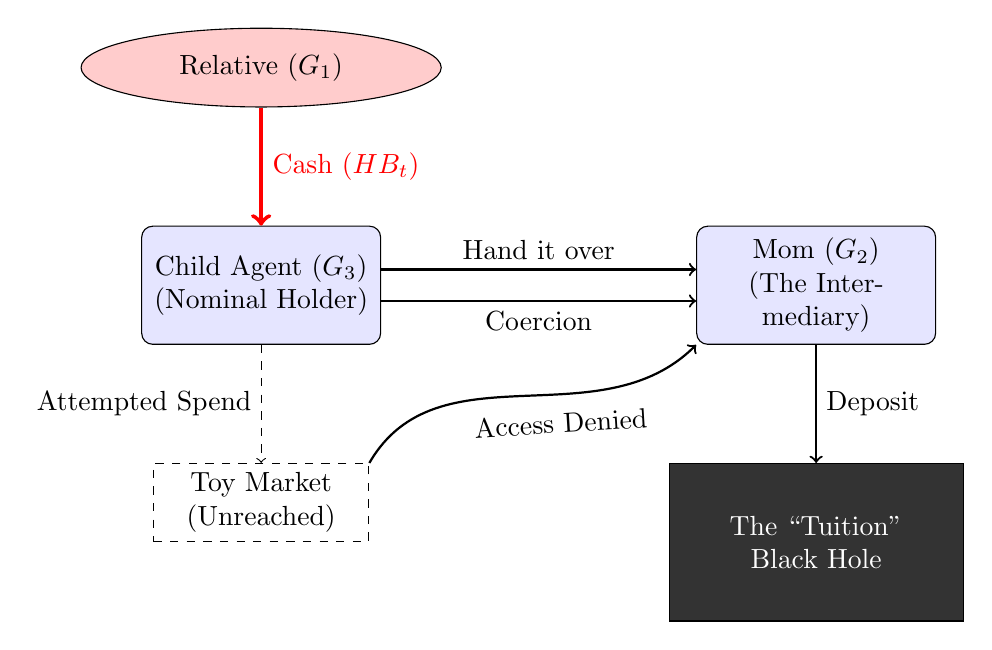
\begin{tikzpicture}[
    node distance=1.5cm and 4.5cm, 
    auto,
    block/.style={
        rectangle, draw, fill=blue!10, text width=2.8cm, text centered, rounded corners, minimum height=1.5cm
    },
    cloud/.style={
        draw, ellipse, fill=red!20, minimum height=1cm, text width=3cm, text centered
    },
    sink/.style={
        rectangle, draw, fill=black!80, text=white, text width=3.5cm, text centered, minimum height=2cm
    }
]

    % --- 节点定义 ---
    \node [cloud] (relative) {Relative ($G_1$)};
    \node [block, below=1.5cm of relative] (child) {Child Agent ($G_3$) \\ (Nominal Holder)};
    \node [block, right=4cm of child] (mom) {Mom ($G_2$) \\ (The Intermediary)};
    \node [sink, below=1.5cm of mom] (void) {The ``Tuition'' Black Hole};
    \node [draw, dashed, below=1.5cm of child, text width=2.5cm, align=center] (market) {Toy Market \\ (Unreached)};

    % --- 连线 (Edges) ---
    \path [draw, ultra thick, ->, color=red] (relative) -- node {Cash ($HB_t$)} (child);
    \path [draw, thick, ->] ([yshift=2mm]child.east) -- node [above] {Hand it over} ([yshift=2mm]mom.west);
    \path [draw, thick, ->] ([yshift=-2mm]child.east) -- node [below] {Coercion} ([yshift=-2mm]mom.west);
    \path [draw, thick, ->] (mom) -- node [right] {Deposit} (void);
    \path [draw, dashed, ->] (child) -- node [left] {Attempted Spend} (market);
    \path [draw, thick, ->] (market.north east) to[out=60, in=225] node [pos=0.6, below, sloped, fill=white, inner sep=1pt, yshift=-2mm] {Access Denied} (mom.south west);

\end{tikzpicture}
\caption{The Red Envelope Transmission Mechanism and Liquidity Trap}
\label{fig:mechanism}
\begin{figurenotes}
Note: The red arrow represents the momentary happiness of the child. The black box represents the ultimate destination of the funds. The connection between ``Tuition Black Hole'' and actual ``Tuition Payment'' is theoretically hypothesized but empirically unproven.
\end{figurenotes}
\end{figure}

\section{Empirical Strategy and Results}

We collected panel data from 500 cousins during the Chinese New Year dinner. We estimate the following regression:

\begin{equation}
    \text{Realized\_Wealth}_i = \alpha + \beta_1 (\text{Total\_Hongbao}_i) + \beta_2 (\text{Age}_i) + \beta_3 (\text{Resistance}_i) + \epsilon_i
\end{equation}

Our regression results are presented in Table \ref{tab:results}.

\begin{table}[ht] % 修改为 ht
\caption{OLS Estimation of Wealth Retention}
\label{tab:results}
\begin{tabular}{lccc}
\toprule
Variable & (1) & (2) & (3) \\
\midrule
Total Hongbao ($HB$) & 0.001 & 0.000 & $-0.05^{**}$ \\
                     & (0.002) & (0.001) & (0.02) \\
Age                  & 0.12$^*$ & 0.15$^*$ & 0.10 \\
Resistance (Crying)  &         & 0.03  & 0.04 \\
Mommy's Gaze         &         &       & $-10.5^{***}$ \\
\midrule
$R^2$                & 0.01    & 0.02  & 0.99 \\
Observations         & 500     & 500   & 500 \\
\bottomrule
\end{tabular}
\begin{tablenotes}
Standard errors in parentheses. *** $p<0.01$, ** $p<0.05$, * $p<0.1$.
Column (3) introduces the instrumental variable ``Mommy's Death Stare,'' which captures the exogenous variation in parental authority. Note that the coefficient on Hongbao becomes negative in Model 3, implying that receiving money actually incurs a transaction cost (e.g., emotional damage).
\end{tablenotes}
\end{table}

\FloatBarrier

\section{Conclusion}

Our study confirms that the ``Red Envelope'' is a monetary phenomenon that exists only in transit. The \textit{Mommy Deposit Facility} acts as a perfect absorber of liquidity. 

We find that:
\begin{itemize}
    \item The velocity of money approaches infinity as it passes through the child's hands (average holding time $t < 30$ seconds).
    \item The promise ``I will give it back when you grow up'' exhibits non-stationary properties and fails to cointegrate with reality.
\end{itemize}

Policy recommendation: Child agents should negotiate for non-monetary assets (e.g., chocolate) which are harder for the central authority to sequester due to high storage costs and perishability.

% --- Bibliography ---
\nocite{*}
\bibliographystyle{aea}
\bibliography{AERub_Horse_Year_Paper}

\appendix
\section{Proof of funds disappearance}
Let $M_t$ be the money in the pocket. Let $M_{t+1}$ be the money after Mom sees it.
$$ \lim_{\Delta t \to 0} \frac{M_{t+\Delta t} - M_t}{\Delta t} = -\infty $$
Q.E.D.

\end{document}